% Intended LaTeX compiler: pdflatex
\documentclass[10pt,a4paper,UTF8]{article}
\usepackage{zclorg}
\usepackage{tikztheorem}
\author{emacsun}
\date{}
\title{对高斯分布的贝叶斯推断}
\hypersetup{
 pdfauthor={emacsun},
 pdftitle={对高斯分布的贝叶斯推断},
 pdfkeywords={},
 pdfsubject={},
 pdfcreator={Emacs 25.0.50.1 (Org mode 9.0.6)},
 pdflang={English}}
\begin{document}

\maketitle
\tableofcontents
\titlepic{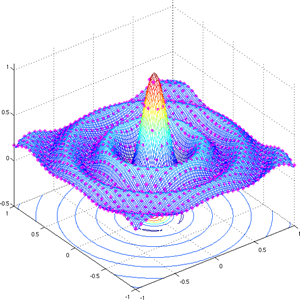
\includegraphics[scale=0.25]{../../img/sinc.PNG}}

\section{简介}
\label{sec:orgac27809}


在最大似然的框架中,我们得到了高斯分布\(\mathbf{\mu}\)和\(\mathbf{\Sigma}\)的点估计。现在,我们采用贝叶斯方法处理这个问题,为此我们需要引入这些参数的先验估计。
\section{假设方差已知}
\label{sec:org0695438}


作为一个例子,我们考虑单个高斯随机变量\(x\),假设方差\(\sigma^{2}\)已知,我们要做的是从\(N\)个观测值\(\mathbf{X} = \{x_{1},\ldots ,x_{N}\}\)中推断出均值\(\mu\)。 似然函数定义为:
\begin{equation}
\label{eq:1}
p(\mathbf{X}|\mu) = \prod_{n=1}^{N}p(x_{n}|\mu) = \frac{1}{(2\pi\sigma^{2})^{N/2}}\exp\bigg\{-\frac{1}{2\sigma^{2}} \sum_{n=1}^{N}(x_{n}-\mu)^{2}\bigg\}
\end{equation}
值得强调的是:似然函数\(p(\mathbf{X}|\mu)\)不是关于\(\mu\)的概率密度函数,并且这个似然函数不是归一化的。

从式(\ref{eq:1})我们可以看出似然函数中\(\mu\)的二次型出现在指数位置上。如果我们选择高斯分布作为\(\mu\)的先验分布\(p(\mu)\)。那么这个高斯分布就是这个似然函数的共轭先验分布,因为对应的后验分布是两个关于\(\mu\)的指数二次型函数的乘积。因此,我们假设\(\mu\)的先验分布为:
\begin{equation}
\label{eq:2}
p(\mu) = \mathcal{N}(\mu|\mu_{0},\sigma_{0}^{2})
\end{equation}
因此后验分布为:
\begin{equation}
\label{eq:3}
p(\mu|\mathbf{X}) \propto p(\mathbf{X}|\mu)p(\mu)
\end{equation}
通过化简我们得到:
\begin{equation}
\label{eq:4}
p(\mu|\mathbf{X}) = \mathcal{N}(\mu|\mu_{N},\sigma_{N}^{2})
\end{equation}
其中:
\begin{eqnarray}
\label{eq:5}
\mu_{N}&=& \frac{\sigma^{2}}{N\sigma_{0}^{2} + \sigma^{2}}\mu_{0} + \frac{N\sigma_{0}^{2}}{N\sigma_{0}^{2} +\sigma^{2}}\mu_{ML} \\
\frac{1}{\sigma_{N}^{2}} &=& \frac{1}{\sigma_{0}^{2}} + \frac{N}{\sigma^{2}}\\
\mu_{ML}&=& \frac{1}{N} \sum_{n=1}^{N}x_{n}
\end{eqnarray}
我们对式 (\ref{eq:5})中的后验均值和方差做简单的分析。首先,我们注意到\(\mu_{N}\)是\(\mu_{0}\)和\(\mu_{ML}\)的一个折中。如果观测到的点数\(N=0\),那么\(\mu_{N}\)就是\(\mu_{0}\)。当\(N\to \infty\)时,\(\mu_{N}\)趋向于\(\mu_{ML}\)。同样的,对于\(\sigma_{N}^{2}\),我们发现使用倒数的表达更清晰易懂。我们称\(\sigma_{N}^{2}\)为方差,称\(\frac{1}{\sigma_{N}^{2}}\)为精度。精度具有可加性,并且后验精度是先验精度加上每一次观测数据的精度。当我们增加观测点数的时候,精度逐渐增加,对应的方差逐渐降低。如果没有观测数据,我们得到的就是先验精度,如果\(N\to \infty\),方差\(\sigma_{N}^{2}\to 0\),此时后验分布会在最大似然解处形成一个无穷高的尖峰。因此,我们通过贝叶斯估计,我们得到了\(\mu\)点估计的最大似然解。注意对于有限的\(N\),如果我们假设\(\sigma_{0}^{2}\to \infty\),那么后验估计\(\mu_{N}\)同样收敛到最大似然解,此时后验方差\(\sigma_{N}^{2} = \sigma^{2}/N\)

我们\href{PRMLch2dot3-maximum-likelihood-for-gaussian.org}{之前} 看到了过高斯分布的均值可以采用迭代的方式计算得出。实际上,贝叶斯估计也可以采用这种方式。
\begin{equation}
\label{eq:6}
p(\mathbf{\mu}| D) \propto \bigg[ p(\mathbf{\mu}) \prod_{n=1}^{N}p(\mathbf{x}_{n}| \mathbf{\mu}) \bigg] p(\mathbf{x}_{N}|\mathbf{\mu})
\end{equation}
式 (\ref{eq:6})中在中括号中的项代表观测到\(N-1\)个数据之后的后验分布。我们看到,这个观测值可以当做第\(N\)次观测的先验分布。实际上,贝叶斯推断的这种序贯视角可以用在任何观测数据是独立同分布的场景中。
\section{假设方差未知}
\label{sec:org9ca01a7}


截止目前,我们的处理手段是方差已知,然后对\(\mu\)做估计。那么,如果方差未知怎么办呢?假设均值已知,我们来估计方差。和本文之前一样,我们也提出一个关于\(\lambda = 1/\sigma^{2}\)的先验估计。关于\(\lambda\)的似然函数可以写为:
\begin{equation}
\label{eq:7}
p(\mathbf{X}|\lambda) = \prod_{n=1}^{N}\mathcal{N}(x_{n}|\mu,\lambda^{-1}) \propto \lambda^{N/2}\exp\bigg\{ -\frac{\lambda}{2} \sum_{n=1}^{N}(x_{n} - \mu)^{2} \bigg\}
\end{equation}
对应的相应的共轭先验应该具有的形式:\(\lambda\)的指数幂乘以\(\lambda\)的线性函数。这样的描述与gamma分布非常类似。gamma分布的定义为:
\begin{equation}
\label{eq:8}
\mathrm{Gam}(\lambda|a,b) = \frac{1}{\Gamma(a)} b^{a}\lambda^{a-1} \exp(-b\lambda)
\end{equation}
这里\(\Gamma(a)\)是gamma函数,出现在这里是为了保证gamma分布是归一化的。gamma分布的期望和方差为:
\begin{eqnarray}
\label{eq:10}
\mathbb{E}[\lambda]&=& \frac{a}{b} \\
\mathrm{var}[\lambda] &=& \frac{a}{b^{2}}
\end{eqnarray}
此处我们考虑先验分布\(\mathbf{Gam}(\lambda|a_{0},b_{0})\),然后我们得到后验概率:
\begin{equation}
\label{eq:11}
p(\lambda|\mathbf{X}) \propto \lambda^{a_{0}-1}\lambda^{N/2}\exp\bigg\{ -b_{0}\lambda -\frac{\lambda}{2}\sum_{n=1}^{N}(x_{n} - \mu)^{2} \bigg\}
\end{equation}
显然,式 (\ref{eq:11})是一个新的gamma分布,参数为\(\mathrm{Gam}(\lambda | a_{N},b_{N})\),其中:
\begin{equation}
\label{eq:12}
a_{N} = a_{0} + \frac{N}{2}
\end{equation}
\begin{equation}
\label{eq:13}
b_{N} = b_{0} + \frac{1}{2}\sum_{n=1}^{N}(x_{n} - \mu)^{2} = b_{0} + \frac{N}{2}\sigma_{ML}^{2}
\end{equation}
其中\(\sigma_{ML}^{2}\)是方差的最大似然估计。

对于式 (\ref{eq:12}),我们发现经过\(N\)次观测之后,\(a\)的值增加了\(N/2\)。因此我们可以把\(a_{0}\)视为\(2a_{0}\)次有效的先验观测。同样,对于式 (\ref{eq:13}),我们发现经过\(N\)次观测,\(b\)的值增加了\(\frac{N}{2}\sigma_{ML}^{2}\)。所以我们可以把\(b_{0}\)解释为先验的\(2a_{0}\)次观测的等效方差\(\tfrac{b_{0}}{a_{0}}\)。
\section{方差和均值都未知}
\label{sec:orge2a9a4b}


当方差和均值都未知时,为了找到一个共轭先验分布,我们考虑\(\mu\)和\(\lambda\)的先验函数:
\begin{equation}
\label{eq:14}
p(\mathbf{X} | \mu,\lambda) = \prod_{n=1}^{N} \bigg(\frac{\lambda}{2\pi} \bigg)^{1/2}\exp \bigg\{ -\frac{\lambda}{2}(x_{n}-\mu)^{2}\bigg\}
\end{equation}
上式可以近似为:
\begin{equation}
\label{eq:15}
\bigg[ \lambda^{1/2}\exp(-\tfrac{\lambda\mu^{2}}{2}) \bigg]^{N}\exp\bigg\{\lambda\mu\sum_{n=1}^{N}x_{n} - \frac{\lambda}{2}\sum_{n=1}^{N}x_{n}^{2}\bigg\}
\end{equation}
我们要找到一个共轭先验分布\(p(\mu,\lambda)\)其形式和式 (\ref{eq:15})类似,即:
\begin{eqnarray}
\label{eq:17}
p(\mu,\lambda)&=& \bigg[ \lambda^{1/2}\exp(-\tfrac{\lambda\mu^{2}}{2}) \bigg]^{\beta} \exp\{c\lambda\mu - d\lambda\} \\
&=&\exp\bigg\{ -\frac{\beta\lambda}{2}(\mu - c/\beta)^{2} \bigg\}\lambda^{\beta/2}\exp\bigg\{ - (d - \frac{c^{2}}{2\beta})\lambda \bigg\}
\end{eqnarray}
其中\(c,d,\beta\)是常量。根据\(p(\mu,\lambda) = p(\mu|\lambda)p(\lambda)\),通过观察式 (\ref{eq:17}),我们令\(p(\mu|\lambda)\)是一个高斯分布,其精度是\(\lambda\)的线性函数;令\(p(\lambda)\)是一个gamma分布。所以:
\begin{equation}
\label{eq:18}
p(\mu,\lambda) = \mathcal{N}(\mu| \mu_{0},(\beta\lambda)^{-1}) \mathrm{Gam}(\lambda|a,b)
\end{equation}
其中,我们定义\(\mu_{0} = c/\beta, a = 1+ \beta/2, b= d-c^{2}/2\beta\)。式 (\ref{eq:18})又被称为正态gamma分布或者高斯gamma分布。注意式(\ref{eq:18})不是简单的正态分布和gamma分布的乘积。因为\(\mu\)的精度是\(\lambda\)的线性函数。即使我们选择了一个先验分布保证\(\mu\)和\(\lambda\)是独立的,在迭代过程中得到的后验分布中\(\mu\)和\(\lambda\)也会纠缠在一起。
\end{document}
